In order to build a dataset containing real-world trajectories, we initially are in need of historical AIS data. Although, the AIS signal from every ship gets freely broadcasted and can be potentially received by anyone with a suitable receiver or antenna, we still struggled to obtain a raw dataset. Services like \textit{MarineTraffic} display live ship positions based on AIS data but getting access to historical data involves a fee and a request which in fact got ignored in our case. Even our friendly request for free historical AIS data for academic use at a local institution, the "Maritime Safety and Security Centre" in Cuxhaven, got denied with a reference to a german law that requires every claimant to pay a fee.
\par
Fortunately, the DLR-MI has access to historical AIS data through a service called \textit{AISHub} which allows its members to exchange AIS data. Thus, our raw dataset consists of four months of raw AIS signals from the year 2020 (first month of each quarter). To be more precise, for the recorded months January, April, July, October over 5,93 million AIS messages are available that got sent by 2011 distinct ships (based on the amount of unique MMSIs). The observation windows is spanned by longitude from $8\degree37.2'N$ to $8\degree59.1'N$ and latitude from $53\degree49.0'W$ to $53\degree71.9'W$.
\par
The process of filtering and extracting single vessel trajectories is done  in  conjunction  with  the  library \textit{MovingPandas} (see chapter \ref{subchap:movingPandas}) and can be summarized by the following steps:
\paragraph{1. Remove unwanted speed records.}
Prior to any conversion to intern class \textit{Trajectory} of MovingPandas, the raw AIS records get filtered by the speed over ground (SOG). The focus of this thesis is on moving ships that enter or leave the port, hence we remove records that indicate that a ship moves too slow ($<3$ knots). Additionally, we remove instances where a ship is speeding or the SOG value is unrealistic for the ship types (passenger, cargo and tanker) we are most interested in ($>30$ knots).


\paragraph{2. Extract provisionally trajectories.}
In the next step, we transform the raw AIS signals to trajectories respectively into a \textit{TrajectoryCollection}, an intern class from MovingPandas which holds multiple trajectories that in return are constructed based on the unique MMSI. 

\paragraph{3. Add artificial direction and speed.}
MovingPandas offers the functionality to add artificial values for the direction and speed purely based on the given geographic positions (longitude and latitude). We will add this information in addition to the SOG and COG values of the AIS signal because we do not use a dedicated ship simulation to calculate next ship positions. It is a matter of testing, if there is any noticable difference in using the artificial values or the values given by the AIS signal. Our assumption is that if we take the positions as ground truth for the calculation of direction and speed by using the functions of MovingPandas, we utilize the exact some transition dynamics when it comes to calculating next ship positions in the custom AIS environment.

\paragraph{4. Remove outliers.}
MovingPandas allows the cleaning of outliers based on the interquartile range. This rather simple approach works by first calculating the range between the first and third quartile. Afterwards, this range is multiplied by a constant $\alpha$ which in our case is $3$ solely because MovingPandas suggests this value in the corresponding function description. The resulting value is subtracted from the first quartile and added to the third quartile. All values outside the range of those two values are marked as outliers and get removed.

\paragraph{5. Split trajectories by time gaps.}
Trajectories are constructed by MovingPandas entirely based on the MMSI. Under the hood, MovingPandas simply groups the input dataframe by the MMSI, which eventually leads to a single trajectory per unique ship. To be able to separate those single trajectories into voyages, MovingPandas offers a variety of \textit{Splitters}. The first \textit{Splitter} we will apply is the \textit{ObservationGapSplitter} which splits trajectories that have too long gaps in consecutive AIS signals. Not only will this operation extract unique voyages of ships, it will also remove disrupted signals which would require long phases of interpolated values.
We chose a minimum time delta per gap of five minutes.

\paragraph{6. Split trajectories by stops.}
Visualizations of the trajectories after the previous step still show ships that do not move towards a destination and are probably anchoring or wait in a floodgate. One example of those unwanted tracks are the tugs that lie in the tug harbour. Their AIS signal is disturbed, resulting in positions that jump arbitrary and thus being recognized as moving. To fix this issue and remove those fake voyages, we apply the \textit{StopSplitter}. This class takes in all tracks and splits them by ships that stay within a predefined area for a minimum duration. In our case, we remove and split ships that stay within an area of 15 meters in diameter for at least three minutes.


\paragraph{7. Remove short trajectories.}
We solely keep trajectories that have a length of more than 1500 meters to  exclude ships that move "inside" the port until reaching the floodgates and to create a dataset consisting predominantly of trajectories documenting the way large ships leave or approach the port from the North Sea.

\paragraph{8. Upsample and unify time intervals.}
Finally, all records of every trajectory get resampled to have fixed time intervals of ten seconds. Missing values are linearly interpolated. The idea behind this upsampling is that the time component gets incorporated directly into the dataset and does not have to be provided in the state representation. Without explicitly knowing, the agent will always take actions that lead to the next state ten seconds into the future.
\par

After the extracting process, the resulting dataset consists of 25,019 trajectories with a subset of 300 voyages being shown in Fig. \ref{fig:tracks}.

\begin{figure}[H]
    \centering
    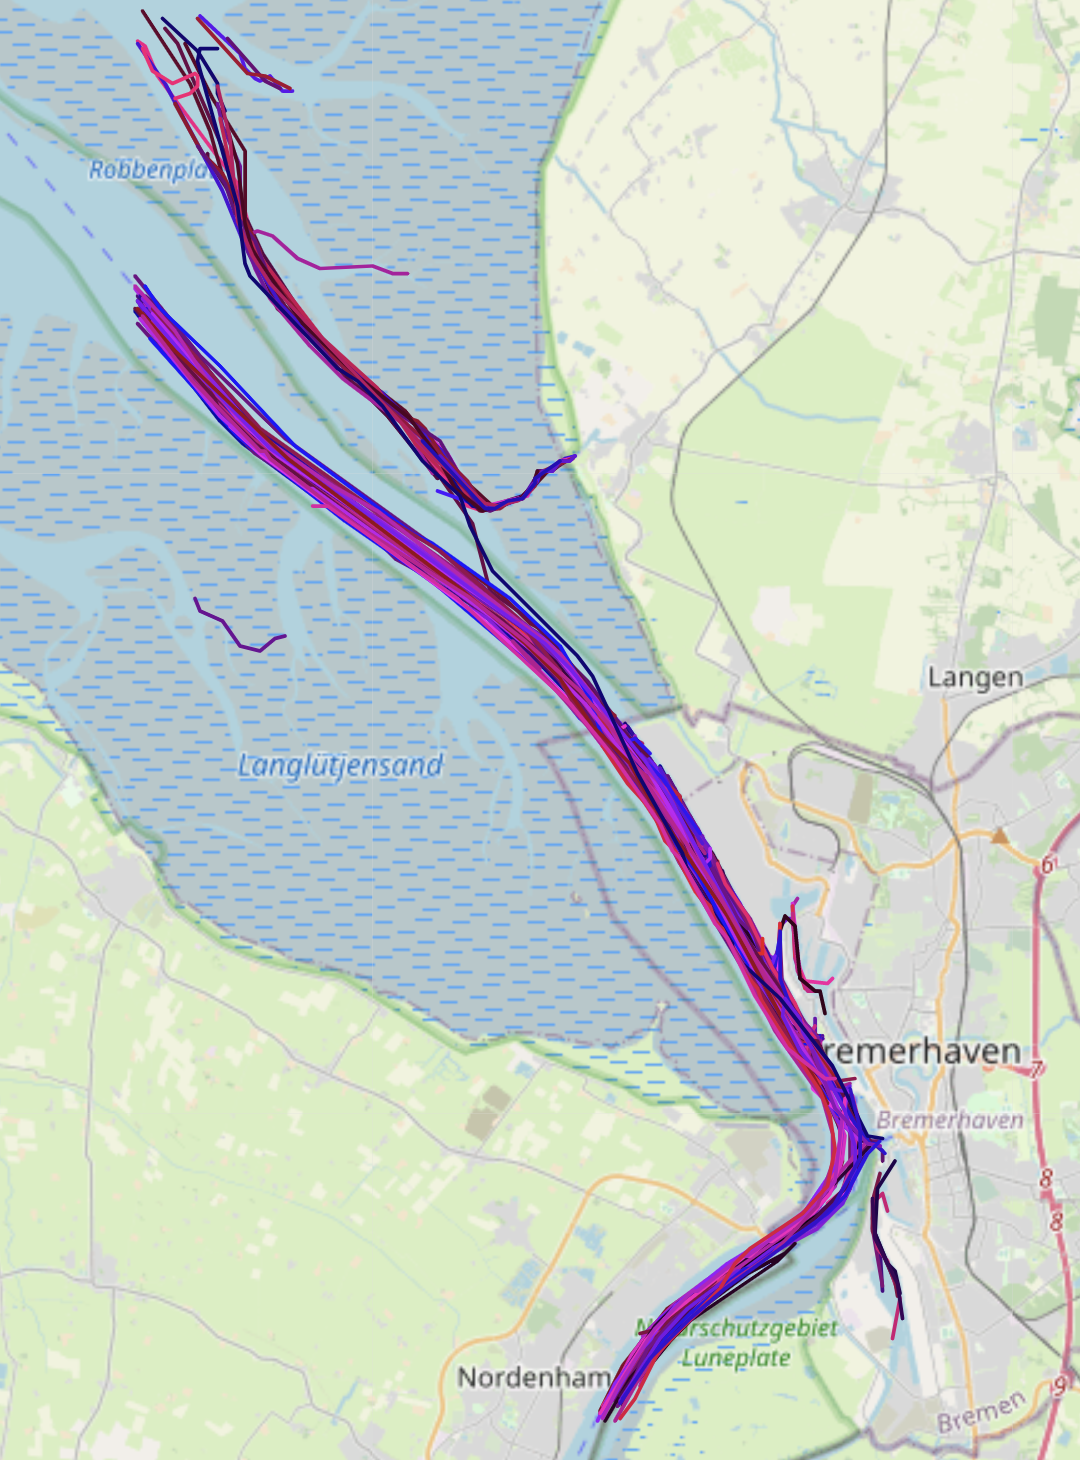
\includegraphics[width=0.5\textwidth]{images/ais/tracks/all_ships.png}
    \caption{Caption}
    \label{fig:tracks}
\end{figure}